\documentclass[review]{elsarticle}

\usepackage{lineno,hyperref}
\usepackage{amsmath,amssymb}
\modulolinenumbers[5]

\journal{Journal of \LaTeX\ Templates}

%%%%%%%%%%%%%%%%%%%%%%%
%% Elsevier bibliography styles
%%%%%%%%%%%%%%%%%%%%%%%
%% To change the style, put a % in front of the second line of the current style and
%% remove the % from the second line of the style you would like to use.
%%%%%%%%%%%%%%%%%%%%%%%

%% Numbered
%\bibliographystyle{model1-num-names}

%% Numbered without titles
%\bibliographystyle{model1a-num-names}

%% Harvard
%\bibliographystyle{model2-names.bst}\biboptions{authoryear}

%% Vancouver numbered
%\usepackage{numcompress}\bibliographystyle{model3-num-names}

%% Vancouver name/year
%\usepackage{numcompress}\bibliographystyle{model4-names}\biboptions{authoryear}

%% APA style
%\bibliographystyle{model5-names}\biboptions{authoryear}

%% AMA style
%\usepackage{numcompress}\bibliographystyle{model6-num-names}

\usepackage[misc]{ifsym}
\usepackage{color}
\usepackage{graphicx}
\usepackage{textcomp}
\usepackage{geometry}

%% `Elsevier LaTeX' style
\bibliographystyle{elsarticle-num}
%%%%%%%%%%%%%%%%%%%%%%%

\begin{document}

\begin{frontmatter}

\title{LAEDNet: A Lightweight Attention Encoder-Decoder Network for Ultrasound Medical Image Segmentation}
% \tnotetext[mytitlenote]{Fully documented templates are available in the elsarticle package on \href{http://www.ctan.org/tex-archive/macros/latex/contrib/elsarticle}{CTAN}.}

%% Group authors per affiliation:
%\author{Elsevier\fnref{myfootnote}}
%\address{Radarweg 29, Amsterdam}
%\fntext[myfootnote]{Since 1880.}

%% or include affiliations in footnotes:
% \author[mymainaddress]{Qianwen Wang}
%\ead[url]{www.elsevier.com}

\author[mymainaddress]{Quan Zhou\corref{mycorrespondingauthor}}
\cortext[mycorrespondingauthor]{Corresponding author}
\ead{quan.zhou@njupt.edu.cn}

\author[mymainaddress]{Qianwen Wang}

\author[mymainaddress]{Yunchao Bao}

\author[mysecondaryaddress]{Lingjun Kong}

\author[mythirdlyaddress]{Xin Jin}

\author[myfourthaddress]{Weihua Ou}

\address[mymainaddress]{National Engineering Research Center of Communications and Networking, \\
Nanjing University of Posts and Telecommunications, Nanjing, China}
\address[mysecondaryaddress]{Faculty of Network and Telecommunication Engineering, Jinling Institute of Technology, Nanjing, China}
\address[mythirdlyaddress]{Department of Computer Science and Technology, 
Beijing Electronic Science and Technology Institute, Beijing, China}
\address[myfourthaddress]{School of Big Data and Computer Science, Guizhou Normal University, Guiyang, China}

\begin{abstract}
Automatic ultrasound image segmentation plays an important role in early diagnosis of human diseases. This paper introduces a novel and efficient encoder-decoder network, called Lightweight Attention Encoder-Decoder Network (LAEDNet), for automatic ultrasound image segmentation. In contrast to previous encoder-decoder networks that involve complicated architecture with numerous parameters, our LAEDNet adopts lightweight version of EfficientNet as encoder. On the other hand, a Lightweight Residual Squeeze-and-Excitation (LRSE) block is employed in decoder. To achieve trade-off between segmentation accuracy and implementing efficiency, we also present a family of models, from light to heavy (denoted as LAEDNet-S, LAEDNet-M, and LAEDNet-L, respectively), with varying lightweight version of EfficientNet backbones. To evaluate LAEDNet, we have conducted extensive experiments on Brachial Plexus Dataset (BP), Breast Ultrasound Images Dataset (BUSI), and Head Circumference Ultrasound Images Dataset (HCUS), where ultrasound images are suffered from high noise, blurred borders and low contrast. The experiments show that, compared with U-Net and its variants, e.g., M-Net, U-Net++ and TransUNet, our LAEDNet achieves better results in terms of Dice Coefficient (DSC) and running speed. Particularly, LAEDNet-M only has 10.75M model parameters with 40.7 FPS, yet obtaining 73.0\%, 73.8\% and 91.3\% DSC on BP, BUSI and HCUS datasets, respectively.
\end{abstract}

\begin{keyword}
\texttt Lightweight network\sep medical ultrasound image segmentation \sep encoder-decoder network\sep visual attention\sep EfficientNet
% \MSC[2010] 00-01\sep  99-00
\end{keyword}

\end{frontmatter}

%\linenumbers

\section{Introduction}

Compared with Magnetic Resonance Imaging (MRI) and Computer Tomography (CT), Ultrasound (US) for diagnosing and analyzing the internal structure of the human body is widely used in the medical field because of its portability, low cost and real-time nature\cite{2018Nerve}. In particular, US is the most common application technique to diagnose brachial plexus neurons and lesions of breast tumors\cite{xue2021global}. Image segmentation is widely used to obtain prominent parts and Regions of Interest (ROI) in medical images, which is conducive to disease diagnosis and pathological follow-up processing. However, due to the inherent characteristics of noise, shadow, speckle, low contrast and blurred edges of ultrasound images, it is a challenge to segment targets from ultrasound images.

Segmentation for ultrasound images has been widely studied in the community of computer vision. Potočnik et al.\cite{Bozidear2002Automated} proposed a hybrid method of spatial constrained kernel fuzzy clustering and edge-based active contour for ultrasonic image segmentation, where a distance regularized level set function is used. Giraldo et al.\cite{HF2015Peripheral} introduced a method based on Bayesian shape model, and the shape prior is initialized by calculating the average shape of the neural structure in the training set. These early attempts rely on prior information to extract features, yet have limited representation ability, leading to the incorrect recognition of lesion regions in complex background.

Recently, the convolutional neural networks (CNNs) have achieved remarkable progress for the task of ultrasound medical image segmentation\cite{ludeep2021,lubrain2018,2019Deep,2020Low,yo2021wide,sun2020image}. Among these networks, the symmetric encoder-decoder architecture like U-Net\cite{2015U} is the mainstream model architecture for medical image segmentation. Recently, a series of U-Net variants\cite{2019Ultrasound,2019Deep,2018Joint,2020UNet} have been proposed to improve performance. For example, M-Net\cite{2018Joint} is an effective modification of U-Net\cite{2015U}, which uses multi-scale inputs and outputs from different levels to monitor the extracted feature maps intensively. Abraham et al.\cite{2019Deep} improved U-Net\cite{2015U} and M-Net\cite{2018Joint} using average pooling instead of maximum pooling to segment brachial plexus. U-Net++\cite{2020UNet} is another powerful encoder-decoder architecture based on U-Net\cite{2015U}, adopting dense connections between each stage of encoder and decoder. TransUNet\cite{chen2021transunet} adopts an architecture which merits both Transformers\cite{vaswani2017attention} and U-Net\cite{2015U} to enhance finer details by recovering localized spatial information. Although these advances have achieved higher segmentation performance, due to the huge amount of model parameters, they are at the cost of expensive computing and low implementing efficiency. However, the execution efficiency of the medical assistance system is crucial in clinical practice. A lightweight network that with a small model size is able to achieve real-time segmentation in a timely fashion (e.g., at least 24 FPS inference speed \footnote{Due to the effect of persistence of vision, human visual system is not sensitive to the change of still images, when they are played at least with 24 FPS \cite{aneja2019real}.}), which is essential for doctors to quickly locate the target position in clinical diagnosis, thus ensuring the smooth progress of treatment, such as anesthetic injection and ultrasonic puncture operation.

In this paper, our goal is to solve the trade-off of accuracy and efficiency as a whole for ultrasound medical image segmentation, rather than just stand on one side. More specifically, our LAEDNet follows the encoder-decoder architecture that is commonly-used for image segmentation tasks. However, medical image segmentation is more challenging since ultrasound images often contains unclear target boundaries and noise background. Intuitively, in the scenario of real-time medical assistance, segmenting ultrasound images not only asks for more powerful encoder backbone to abstract high-level features, but also requires lightweight decoder to integrate extracted features from encoder and recover feature resolutions. Following this principle, on one hand, the encoder of our LAEDNet adopts various lightweight version of EfficientNet \cite{2019EfficientNet} to enhance feature extraction, while keeping low computational costs. Unlike traditional networks (e.g.,U-Net \cite{2015U}, U-Net++ \cite{2020UNet}, and TransUNet \cite{chen2021transunet}) that employs simple concatenation operation to fuse encoder cues, on the other hand, our decoder adopts a lightweight information integration module with the guidance of attention scheme, called LRSE, to recover feature resolutions step-by-step, where deconvolution features are coupled with corresponding encoder counterparts, leading to produce more accurate segmentation results and more smoother object contours. We evaluate our LAEDNet on three challenging datasets, Brachial Plexus Dataset (BP)\cite{Kaggle}, Breast Ultrasound Images Dataset (BUSI)\cite{2019Dataset}, and Head Circumference Ultrasound Images Dataset (HCUS)\cite{2018Automated}. The experimental results show that our method is able to obtain available trade-off in terms of segmentation accuracy and implementing efficiency. In summary, the main contributions of our paper are three-fold: 
\begin{itemize}
\item The asymmetric architecture of LAEDNet leads to the great reduction of network parameters, which accelerates the inference process.
\item We design a lightweight decoder block, LRSE, with the guidance of attention scheme, which can be well coupled with LAEDNet backbone.
\item We test LAEDNet on BP\cite{Kaggle}, BUSI\cite{2019Dataset}, and HCUS\cite{2018Automated}. The comprehensive experiments demonstrate that our LAEDNet-M achieves best trade-off between segmentation accuracy and running efficiency. Particularly, LAEDNet-M only has 10.75M model parameters with 40.7 FPS, yet obtaining 73.0\%, 73.8\% and 91.3\% DSC on BP\cite{Kaggle}, BUSI\cite{2019Dataset} and HCUS\cite{2018Automated}, respectively.
\end{itemize}
 
The remainder of this paper is organized as follows. We first review related work in Section 2, and then elaborate on the details of our LAEDNet in Section 3. Experimental results are demonstrated in Section 4. Results of the ablation experiments are discussed in Section 5. Finally, the conclusion and future work are given in Section 6.

\section{Related work}

In this section, we review the related advances for US medical image segmentation using encoder-decoder architecture. As ultrasound medical image segmentation and visual attention are most related fields to our work, we review the related approaches in these two directions.

\subsection{Ultrasound medical image segmentation}

The recent mainstream approaches prefer to design high accurate networks for ultrasound medical image segmentation. As a pioneer work, U-Net\cite{2015U} designs a mirrored architecture for medical image segmentation. Amiri et al. \cite{2020fine-tuning} fine-tune the shallow layers rather than deep layers in ultrasound image segmentation. The NAS-Unet \cite{2019Nas-unet} is constructed based on a U-like backbone \cite{2015U} to medical image segmentation through neural architecture search. This method needs to manually propose rules of searching space, thus increasing the complexity of network design. To segment regions of breast masses with different size and shape, Michal et al.\cite{2020breastmass} develop a selective kernel U-Net, integrating the merit of dilated convolution and attention module to adaptively enlarge receptive fields. To capture context information, FC-DenseNet\cite{wu2019cascaded} replaces each upsampling and downsampling layer of U-Net\cite{2015U} for kidney segmentation in US Images. Wu et al.\cite{wu2017cascaded} cascade fully convolutional network for prenatal US image segmentation. In order to learn long-range spatial context of transvaginal US image segmentation, CR-Unet\cite{li2019cr} incorporates the spatial recurrent neural network (RNN)\cite{hochreiter1997long} into a plain U-Net\cite{2015U}. Yang et al.\cite{yang2018towards} adopts the RNN in the decoder of U-Net\cite{2015U} to segment prenatal volumetric US image. In DeepNerve\cite{horng2020deepnerve}, RNN is embedded into the encoder for median nerve US image segmentation. Although these methods have made remarkable progress for ultrasound medical image segmentation, they are inevitable to slow down the inference speed because of their huge network model size, which is not suitable for assisting urgent clinical tasks in timely fashion. Conversely, our LAEDNet adopts lightweight version of EfficientNet\cite{2019EfficientNet} as encoder, and designs a set of lightweight attention blocks in decoder, achieving trade-off between segmentation accuracy and implementing efficiency.

Recently, there are two directions of designing a real-time segmentation network: (1) optimizing existing high-accuracy networks, such as pruning \cite{wen2016learning,li2018constrained}, quantization \cite{wu2016quantized,nan2019deep}, and distillation \cite{liu2019structured,qin2021eff,ho2020utilize}, and (2) designing compact lightweight networks, such as LEDNet \cite{wang2019lednet} and AGLNet \cite{zhou2020aglnet}. Although there are a vast number of compact networks designed for semantic segmentation, to our best knowledge, there are few researches that study the medical imaging problems. Some early attempts \cite{qin2021eff,ho2020utilize,jha2021real} have started paying attention to real-time medical image segmentation. Yet there is still a dilemma that the performance tends to be damaged when the models are simplified only for faster speed. In contrast, our LAEDNet belongs to the second category, which seeks best trade-off between accuracy and efficiency for ultrasound medical image segmentation with the guidance of attention scheme.

\subsection{Visual attention}

The recent visual attention used in ultrasound medical image segmentation can be roughly divided into three categories: squeeze attention \cite{woo2018cbam,2017Squeeze}, self-attention \cite{2018non}, and transformers \cite{vaswani2017attention}.
	
The first category often utilizes global average pooling to produce channel or spatial attention used to reweight original feature maps \cite{woo2018cbam,2017Squeeze}. For example, AttentionNet\cite{li2019attentionnet} embeds the spatial attention refinement (SAR) block into backbone to extract more informative features for breast US images segmentation. ReAgU-Net \cite{ding2019automatic} employs the attention gate (AG) to reweight feature maps obtained from shallow layers and deep layers for thyroid US image segmentation. Wang et al.\cite{wang2019deep} adopt the layer-wise attention mechanism to selectively leverage the complementary features across all scales. In contrast, the second category \cite{2018non,2021global} encodes global context by computing correlation matrix of image elements, showing more powerful representation ability with respect to squeeze attention scheme. For instance, Xue et al.\cite{2021global} not only consider channel-wise attention, but also embed long-range spatial dependencies. LEDNet \cite{wang2019lednet} and AGLNet \cite{zhou2020aglnet} adopt additional spatial attention and feature pyramid attention in decoder, yet both channel attention and spatial attention are not designed in a lightweight way. Transformer \cite{vaswani2017attention,chen2021transunet,2021swin}, derived from nature language processing, begins to show their potential for ultrasound image segmentation. For instance, TransUNet \cite{chen2021transunet} attempts to combine the metric of Transformers \cite{vaswani2017attention} and U-Net \cite{2015U} for medical image segmentation. In sprite of having powerful ability to capture global context, these attention models once again are at sacrifice of very large network size, resulting in low implementing efficiency. Unlike these approaches, our goal is to design a lightweight attention	module, called LRSE, to achieve accurate segmentation outputs, while maintaining fast segmenting speed.

\section{Method}

\subsection{Overall network architecture}

\begin{figure}[!t]
	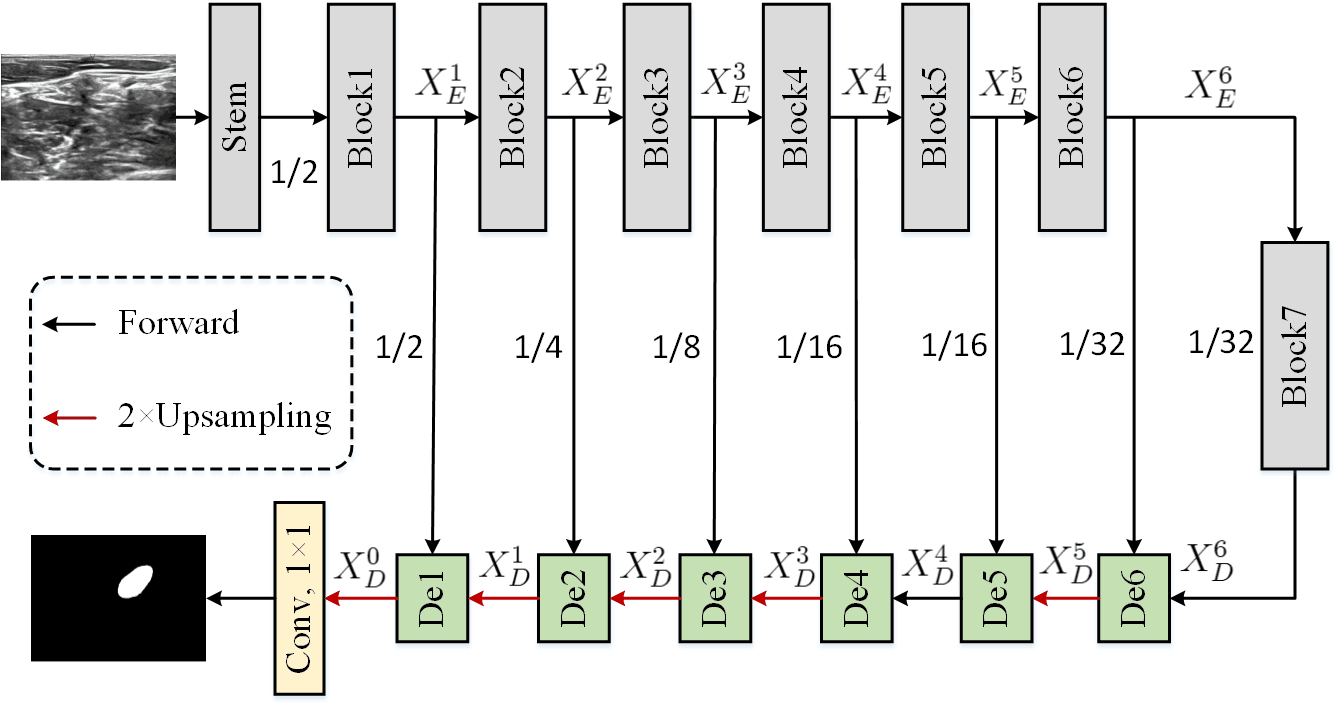
\includegraphics[width=\textwidth]{overall-architecture.png}
	\caption{The overall network architecture of LAEDNet. The gray blocks are a series of encoding modules, and the green blocks represent LRSEs. The black arrows denote information flow, and red arrows indicate 2 times upsampling operation. Note that the entire network has an asymmetrical architecture, as the detail structure in LRSEs is different with convolution stages in encoder. (Best viewed in color)}
	\label{fig1}
\end{figure}

The overall network architecture is shown in Figure \ref{fig1}. LAEDNet also adopts the encoder-decoder architecture similar to U-Net\cite{2015U}, but the specific details of the encoder and the decoder are asymmetrical.

The contraction path of LAEDNet employs an efficient backbone, EfficientNet\cite{2019EfficientNet}, as encoder to reduce model size while extract robust features. There are a total of 8 stages (denoted as gray blocks) in the encoder. The output resolution of stem stage is 1/2 of the input image. Except first stem block, let $X_{E}^{i}$ be the output of the \emph{i}-th block in encoder, then the output resolution of each individual block is 1/2, 1/4, 1/8, 1/16, 1/16, 1/32 and 1/32 with respect to the size of original image. On the other hand, there are six green blocks (LRSE) in the decoder, where feature resolutions are sequentially recovered.

Let $X_{D}^{j-1}$ be the output of the \emph{j}-th LRSE. As can be seen, the \emph{j}-th LRSE has two inputs, $X_{D}^{j}$ from deeper LRSE, and $X_{E}^{i}$ from the counterpart in encoder. Note the feature resolutions are required to be upsampled (indicated as red arrows) for exact integration in each LRSE. Finally, an $1\times1$ convolution is adopted to project feature maps to semantic space. Immediately below, we elaborate on the details of encoder and decoder, respectively.

\subsection{Encoder}

\begin{figure}[!t]
	\centering
	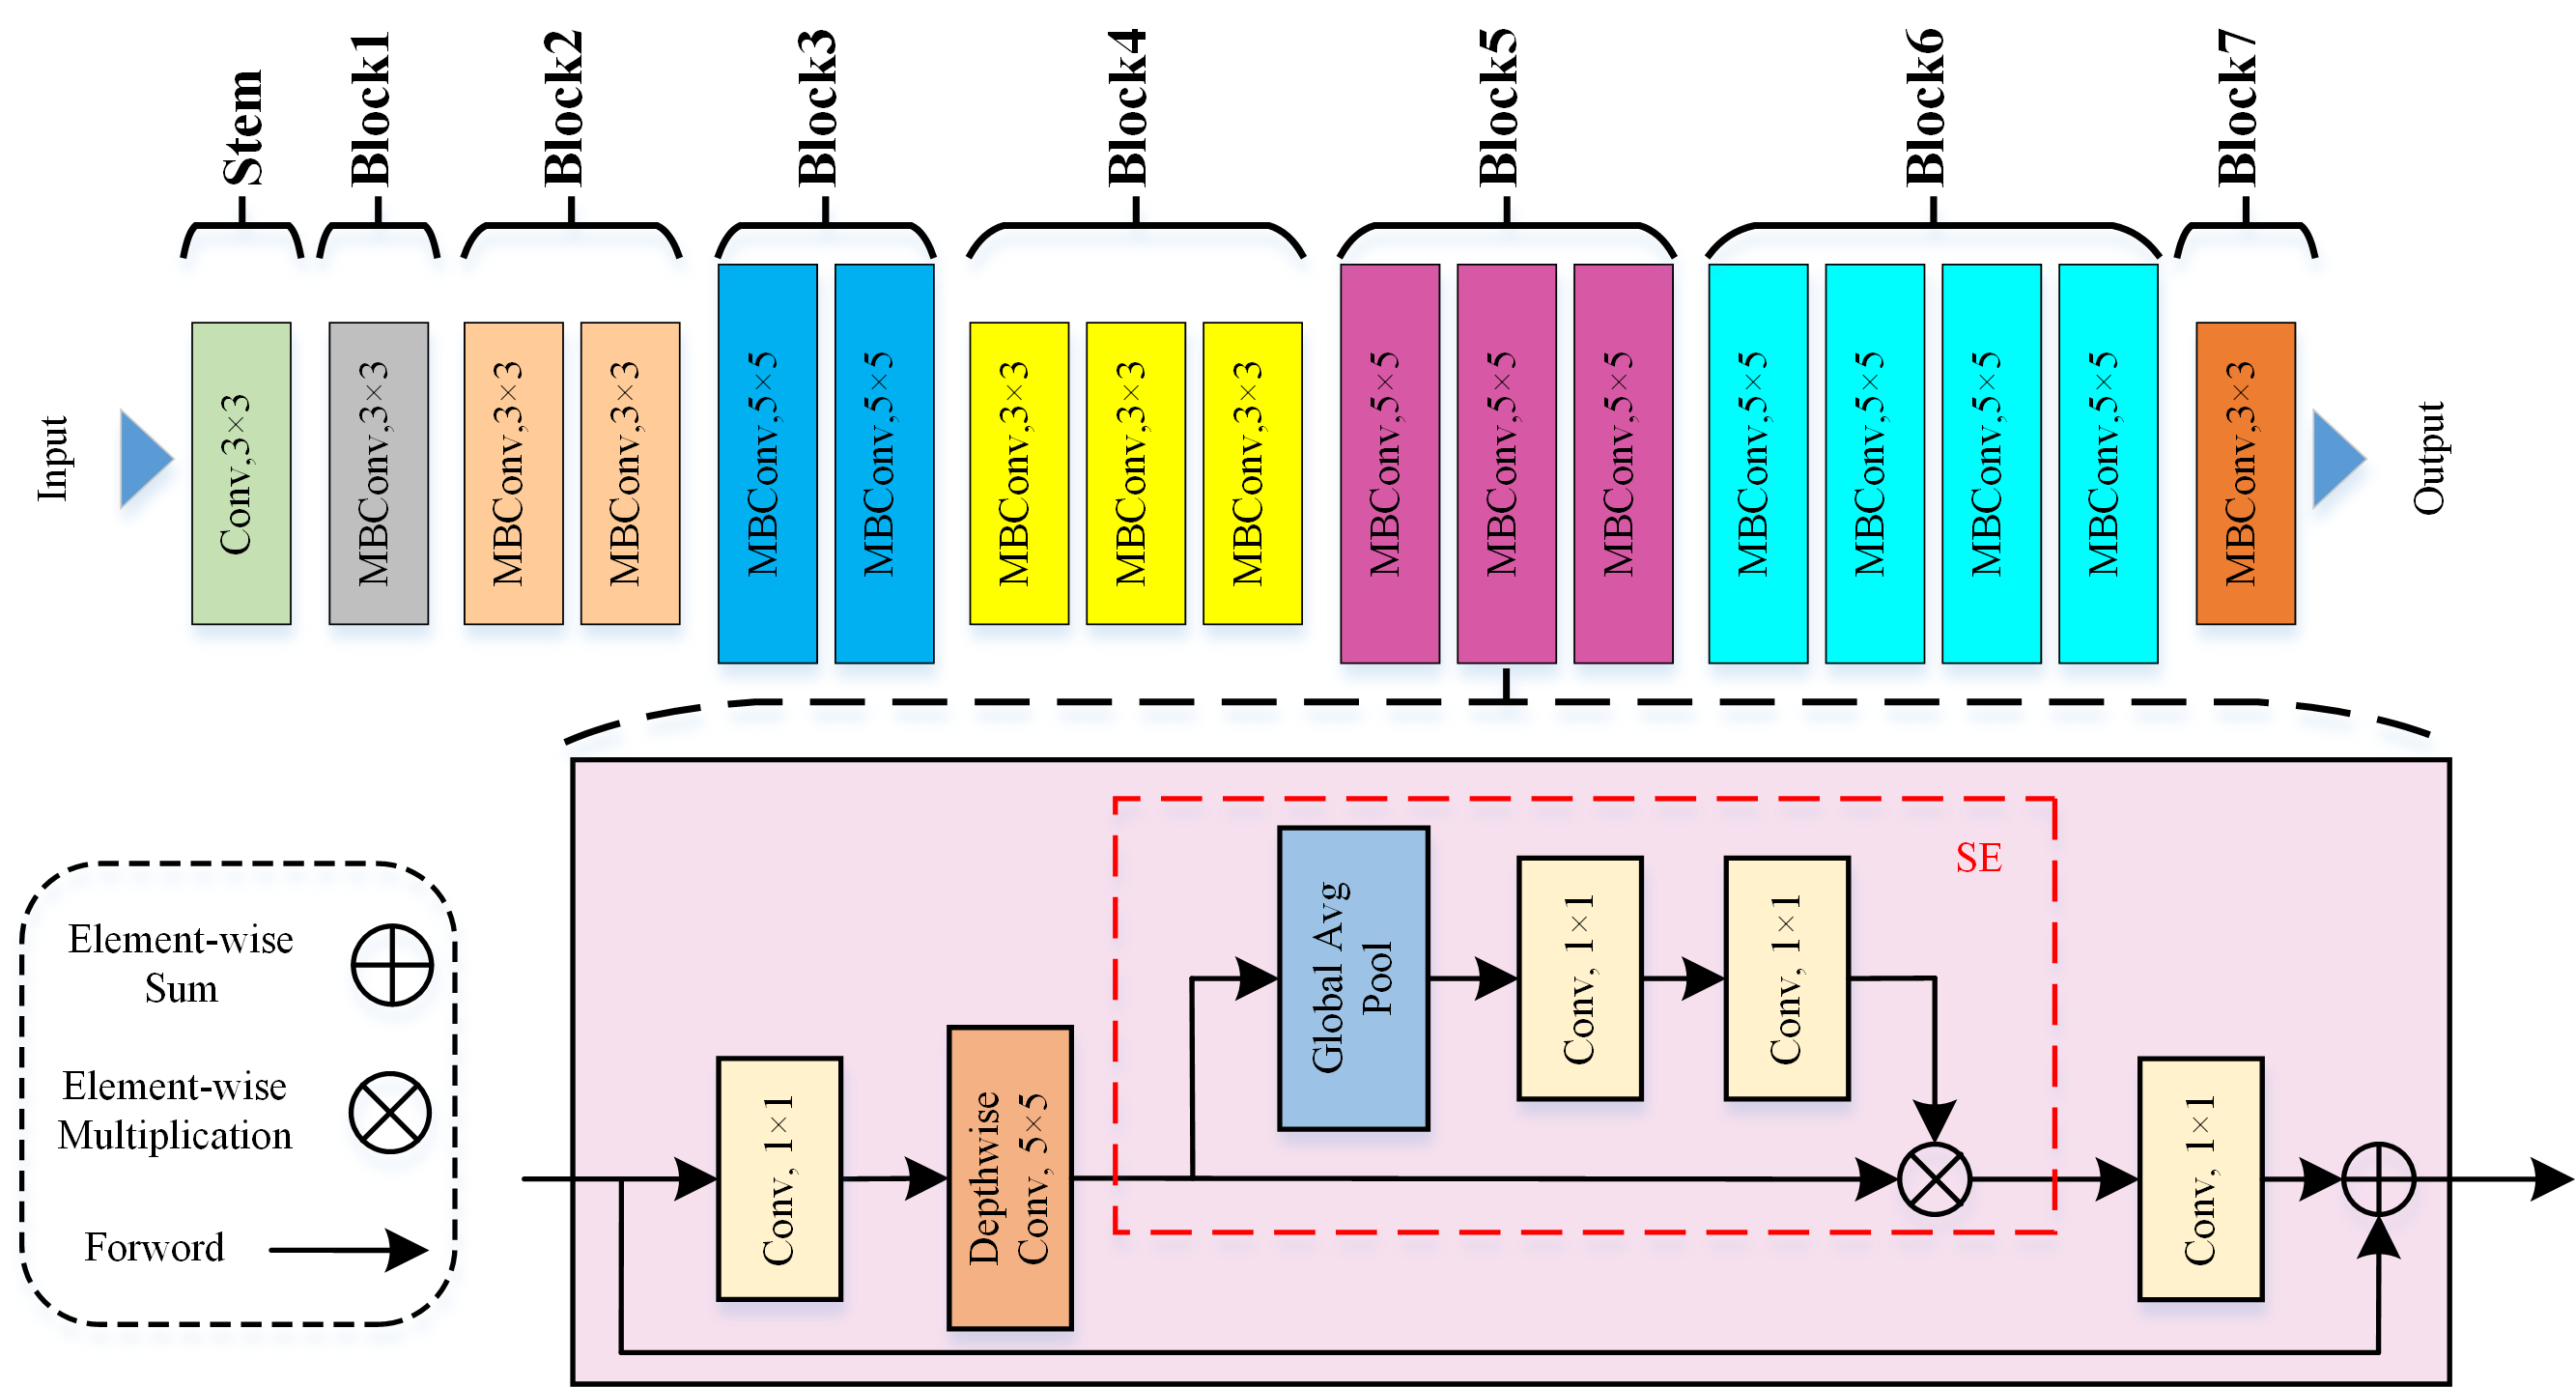
\includegraphics[width=\textwidth,height=0.45\textheight]{Encoder3.png}
	\caption{The structure of encoder in LAEDNet. Different blocks are denoted by different colors. The details of the structure of MBConv are described in the purple block. (Best viewed in color)}
	\label{fig2}
\end{figure}

To achieve performance balance in terms of segmentation accuracy and implementing efficiency, LAEDNet employs three versions of EfficientNet\cite{2019EfficientNet} architecture, EfficientNet-B0, EfficientNet-B3, and EfficientNet-B7 (denoted as LAEDNet-S, LAEDNet-M, and LAEDNet-L, respectively), where the model size is scaled by the number of convolution layers. For convenient understanding, Figure \ref{fig2} takes LAEDNet-S as an example to show the detail structure of backbone. The entire backbone is composed of a stem and a series of convolution blocks, where each block includes a set of repeatably MBConv modules with different size of depthwise convolutions. The MBConv adopts inverted residual architecture that feature channels are first expended and reweighed by squeeze-and-excitation (denoted as red dash line bounding box). Finally, the channel number of reweighed features are reduced for residual connection.

\begin{table}[!t]
	\caption{Detailed encoder architecture of LAEDNet-S, LAEDNet-M, and LAEDNet-L.}
	\centering
	\resizebox{\textwidth}{!}{
		\begin{tabular}{|c|c|c|c|c|}
			\hline
			Layer name & Output size & LAEDNet-S & LAEDNet-M & LAEDNet-L \\
			\hline
			Stem & 160×160 & $[3\times 3,32]\times 1$ & $[3\times 3,40]\times 1$ & $[3\times 3,64]\times 1$\\
			\hline
			Block1 & 160×160 & 
			$\begin{bmatrix}
			DW 3\times 3, 32\\ 
			SE\\ 
			1\times 1, 16
			\end{bmatrix}\times 1$ &
			$\begin{bmatrix}
			DW 3\times 3, 40\\ 
			SE\\ 
			1\times 1, 24
			\end{bmatrix}\times 1$ &
			$\begin{bmatrix}
			DW 3\times 3, (64,32)\\ 
			SE\\ 
			1\times 1, 32
			\end{bmatrix}\times 4$
			\\
			\hline
			Block2 & 80×80 & 
			$\begin{bmatrix}
			1\times 1, (96,144) \\
			DW 3\times 3, (96,144) \\ 
			SE\\ 
			1\times 1, 24
			\end{bmatrix}\times 2$ &
			$\begin{bmatrix}
			1\times 1, (144,192) \\
			DW 3\times 3, (144,192) \\ 
			SE\\ 
			1\times 1, 32
			\end{bmatrix}\times 2$ &
			$\begin{bmatrix}
			1\times 1, (192,288) \\
			DW 3\times 3, (192,288) \\ 
			SE\\ 
			1\times 1, 48
			\end{bmatrix}\times 7$
			\\
			\hline
			Block3 & 40×40 & 
			$\begin{bmatrix}
			1\times 1, (144,240) \\
			DW 5\times 5, (144,240) \\ 
			SE\\ 
			1\times 1, 40
			\end{bmatrix}\times 2$ &
			$\begin{bmatrix}
			1\times 1, (192,288) \\
			DW 5\times 5, (192,288) \\ 
			SE\\ 
			1\times 1, 48
			\end{bmatrix}\times 2$ &
			$\begin{bmatrix}
			1\times 1, (288,480) \\
			DW 5\times 5, (288,480) \\ 
			SE\\ 
			1\times 1, 80
			\end{bmatrix}\times 7$
			\\
			\hline
			Block4 & 20×20 & 
			$\begin{bmatrix}
			1\times 1, (240,480) \\
			DW 3\times 3, (240,480) \\ 
			SE\\ 
			1\times 1, 80
			\end{bmatrix}\times 3$ &
			$\begin{bmatrix}
			1\times 1, (288,576) \\
			DW 3\times 3,(288,576) \\ 
			SE\\ 
			1\times 1, 96
			\end{bmatrix}\times 5$ &
			$\begin{bmatrix}
			1\times 1, (480,960) \\
			DW 3\times 3, (480,960) \\ 
			SE\\ 
			1\times 1, 160
			\end{bmatrix}\times 10$
			\\
			\hline
			Block5 & 20×20 & 
			$\begin{bmatrix}
			1\times 1, (480,672) \\
			DW 5\times 5, (480,672) \\ 
			SE\\ 
			1\times 1, 112
			\end{bmatrix}\times 3$ &
			$\begin{bmatrix}
			1\times 1, (576,816) \\
			DW 5\times 5, (576,816) \\ 
			SE\\ 
			1\times 1, 136
			\end{bmatrix}\times 5$ &
			$\begin{bmatrix}
			1\times 1, (960,1344) \\
			DW 5\times 5, (960,1344) \\ 
			SE\\ 
			1\times 1, 224
			\end{bmatrix}\times 10$
			\\
			\hline
			Block6 & 10×10 & 
			$\begin{bmatrix}
			1\times 1, (672,1152) \\
			DW 5\times 5, (672,1152) \\ 
			SE\\ 
			1\times 1, 192
			\end{bmatrix}\times 4$ &
			$\begin{bmatrix}
			1\times 1, (816,1392) \\
			DW 5\times 5, (816,1392) \\ 
			SE\\ 
			1\times 1, 232
			\end{bmatrix}\times 6$ &
			$\begin{bmatrix}
			1\times 1, (1344,2304) \\
			DW 5\times 5, (1344,2304) \\ 
			SE\\ 
			1\times 1, 384
			\end{bmatrix}\times 13$
			\\
			\hline
			Block7 & 10×10 & 
			$\begin{bmatrix}
			1\times 1, (1152,1920) \\
			DW 3\times 3, (1152,1920) \\ 
			SE\\ 
			1\times 1, 320
			\end{bmatrix}\times 1$ &
			$\begin{bmatrix}
			1\times 1, (1392,2304) \\
			DW 3\times 3, (1392,2304) \\ 
			SE\\ 
			1\times 1, 384
			\end{bmatrix}\times 1$ &
			$\begin{bmatrix}
			1\times 1, (2304,3840) \\
			DW 3\times 3, (2304,3840) \\ 
			SE\\ 
			1\times 1, 640
			\end{bmatrix}\times 4$
			\\
			\hline
		\end{tabular}\label{table1}
	}
\end{table}

More specifically, the detailed encoder structure of LAEDNet-S, LAEDNet-M, and LAEDNet-L are exhibits in Table \ref{table1}. The input size of the image is $320\times320\times3$, and the output size of each block sequentially decreases along with going deeper of entire network. All three types of encoders are stacked by a stem layer and 7 convolution blocks. Specifically, the stem block is a convolution layer using $3\times3$ filtering with stride 2, which reduce the dimension of the input image. The next 7 blocks consist of a set of mobile inverted bottlenecks (MBConvs)\cite{2018MobileNetV2} with the squeeze-and-excitation (SE)\cite{2017Squeeze} optimization. In different lightweight version of LAEDNet, MBConv is repeated with different times, leading to different number of convolution layers and model size. Considering LAEDNet-S as an example, MBConvs are repeated \emph{m} times in each convolution block, where different block stages has different structures of MBConv. In each MBConv, an $1\times1$ convolution is first applied to increase the number of feature channels to (\emph{c}$_{1}$,\emph{c}$_{2}$), where \emph{c}$_{1}$ is only used for first MBConv in each block, and the rest MBConvs adopt \emph{c}$_{2}$. Thereafter, a depthwise convolution is performed with $3\times3$ filter kernel size. The filtering feature maps are reweighted by the forthcoming SE attention module. Finally, another $1\times1$ convolution is employed to reduce feature dimensions, where the output feature maps are fed into next MBConv. Compared with LAEDNet-S, LAEDNet-M, and LAEDNet-L adopt similar architecture, yet have different number of filter feature channels and repeated times \emph{m} of MBConv.

\subsection{Decoder}

\begin{figure}[!t]
	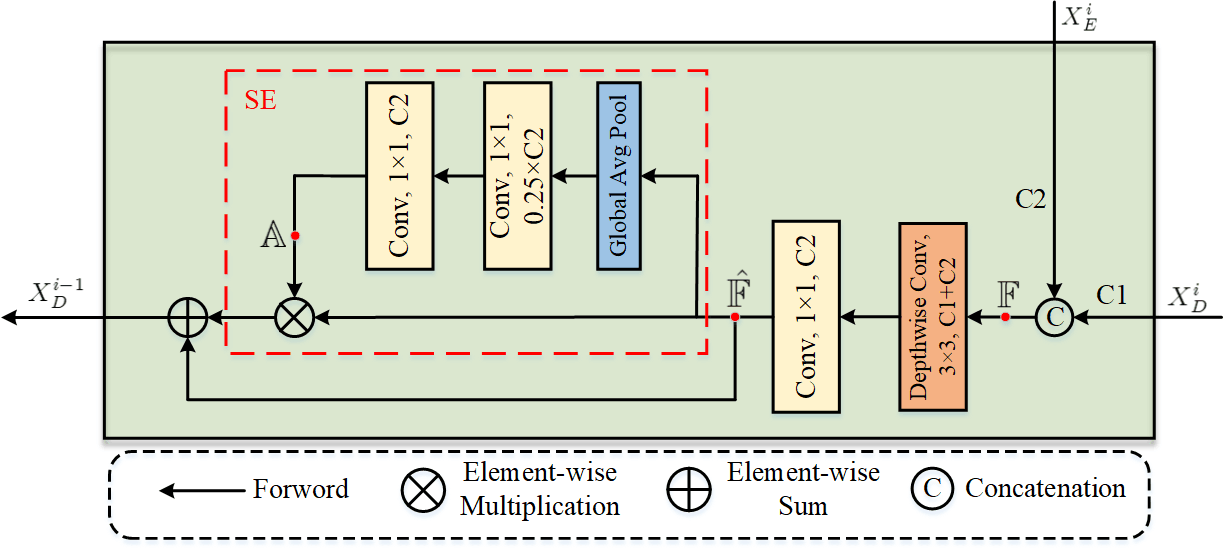
\includegraphics[width=\textwidth]{LRSE-Decoder.png}
	\caption{Illustration of LRSE. The orange, yellow, and blue module represent the depthwise convolution, 1×1 convolution and global average pooling, respectively. (Best viewed in color)}
	\label{fig3}
	\end{figure}

The detailed architecture of LRSE used in decoder is depicted in Figure 3, where LRSE makes the decoder well coupled with the encoder. For \emph{i}-th LRSE in decoder, it integrates the upsampled features $X_{D}^{i}\in \mathbb{R^{\mathrm{W\times H\times C1}}}$ from previous LRSE, and the counterpart feature maps $X_{E}^{i}\in \mathbb{R^{\mathrm{W\times H\times C2}}}$ in encoder to produce output features $X_{D}^{i-1}\in \mathbb{R^{\mathrm{W\times H\times C2}}}$. Note, as shown in Figure \ref{fig1}, there is no need to upsample $X_{D}^{4}$ and $X_{D}^{6}$, as they already have the same resolution with respect to the corresponding $X_{E}^{4}$ and $X_{E}^{6}$. Specifically, we first fuse $X_{D}^{i}$ and $X_{E}^{i}$ by concatenation:

\begin{equation}
	\mathbb{F}=[X_{D}^{i}, X_{E}^{i}]
\end{equation}
where $[\cdot]$ denotes concatenated operation. Then, the produced features $\mathbb{F}\in \mathbb{R^{\mathrm{W\times H\times (C1+C2)}}}$ are fed into a $3\times3$ depthwise convolution, where each feature channel is convoluted independently. To construct correlations among feature channels, an $1\times1$ convolution is applied, and the feature dimension is reduced at the same time. Let $\textup{F}_{l}$ be these lightweight convolution operations, and $\theta _{l}$ is the associated parameters. Then the output features $\hat{\mathbb{F}}\in \mathbb{R^{\mathrm{W\times H\times C2}}}$ can be calculated as:

\begin{equation}
	\hat{\mathbb{F}}=\textup{F}_{l}(\mathbb{F},\theta _{l})
\end{equation}
The final step of LRSE is reweighting $\hat{\mathbb{F}}$ with the guidance of SE\cite{2017Squeeze} attention. To this end, an average pooling is first used to squeeze input feature $\hat{\mathbb{F}}$ into a one-dimensional vector, then two $1\times1$ convolutions are employed to produce a channel-wised attention map $\mathbb{A}\in \mathbb{R^{\mathrm{1\times 1\times C2}}}$:
\begin{equation}
	\mathbb{A}=\textup{F}_{SE}(\textbf{avg}(\hat{\mathbb{F}}),\theta _{SE})
\end{equation}
where $avg(\cdot)$ is an average pooling operation, $\textup{F}_{SE}$ indicates projection using $1\times1$ convolutions and $\theta _{SE}$ is the associated parameters. Finally, the output $X_{D}^{i-1}\in \mathbb{R^{\mathrm{W\times H\times C2}}}$ is calculated by combined features $\hat{\mathbb{F}}$ and its reweighted counterpart:
\begin{equation}
	X_{D}^{i-1}=\hat{\mathbb{F}}+\mathbb{A}\bigotimes \hat{\mathbb{F}}
\end{equation}
where $\bigotimes$ stands for element-wise multiplication, and an identity mapping is used to leverage model training and feature reweighting. 

Note SE is both used in encoder and decoder of LAEDNet, yet it has different effects. In encoder, SE is part of MBConv, and used to reweight feature maps with expanded channels. In decoder, on the contrary, SE is used to reweight integrated feature maps, derived from previous deconvolution features and the encoder counterpart.

\section{Experiments}

To demonstrate the effectiveness and scalability of LAEDNet, we have conducted extensive experiments for different medical segmentation scenarios: BP\cite{Kaggle} for neck, BUSI\cite{2019Dataset} for chest, and HCUS\cite{2018Automated} for fetal head in the womb. The experimental results show that our LAEDNet achieves best balance between segmentation accuracy and implementing efficiency on these datasets.

\subsection{Dataset}\label{dataset}

BP \cite{Kaggle} dataset (\url{https://www.kaggle.com/c/ultrasound-nerve-segmentation}) was released by Kaggle competition in 2016. It consists of 5635 ultrasound images of brachial plexus neurons from 47 patients, including 2323 images with neuron targets and 3312 images without neuron targets. For each patient, about 120 images were collected. The resolution of all original images are $420\times580$. In data pre-processing, we divide the entire dataset into training set and validation set according to the ratio of 9:1. Specifically, to ensure the same sample distribution between the training set and the validation set, we construct validation set using 1/10 of the images with and without neuron targets. The rest of the images are used to form training set.

BUSI \cite{2019Dataset} dataset (\url{https://scholar.cu.edu.eg/?q=afahmy/pages/dataset}) was collected in 2018 and includes breast ultrasound images of 600 women aged 25 to 75. The dataset consists of 780 images in PNG format, with an average image size of $500\times500$ pixels. The images in BUSI\cite{2019Dataset} are divided into three categories: normal, benign and malignant, with 133, 437 and 210 images, respectively. Similar to data splitting scheme used in BP\cite{Kaggle}, we divide the images of these three categories in the ratio of 8:2 (training vs testing) in our experiments.

HCUS \cite{2018Automated} dataset (\url{https://hc18.grand-challenge.org/}) was from a grand challenge 2018 for fetal head segmentation. It contains 999 ultrasound images of the fetus head circumference. The corresponding ground truth are produced by a trained sonographer. The size of each 2D ultrasound image is $800\times540$ pixels. We divide the dataset into a training set of 800 images and a test set of 199 images in the ratio of 8:2.

\subsection{Evaluation metrics and baselines}

We adopt Dice score (DSC), Intersection-over-Union (IoU), and Area under curve (AUC) to measure segmentation accuracy, while Frames Per Second (FPS) and model size are used to evaluate implementing efficiency. For BP\cite{Kaggle}, we also calculate the Leaderboard Score (LB DSC)\cite{Kaggle} of test set, provided by the Kaggle competition website, to evaluate our method. The calculation formula of LB DSC is the same as DSC, which is defined as:
\begin{equation}
	DSC=\frac{2\left | X\cap Y \right |}{\left | X \right |+\left | Y \right |}
\end{equation}
where \emph{X} is the segmentation result and \emph{Y} is the ground truth. 

In order to show the superiority of LAEDNet, we select U-Net\cite{2015U}, M-Net\cite{2019Deep}, U-Net++\cite{2020UNet}, SK-U-Net\cite{2020breastmass}, and TransUNet\cite{chen2021transunet} as the baselines for comparison.

\subsection{Implementation}

The models are implemented using Keras framework and trained with a NVIDIA GeForce GTX 1080 GPU. The input images are all resized to $320\times320$ pixels for three datasets. The Adam optimizer\cite{2015Adam} is used with a learning rate of $1\times 10^{-4}$. For fair comparison, statistical tests are conducted to evaluate our model. Specifically, we randomly exchange images between training and validation set, but holding data splitting criteria in each dataset. Then our LAEDNet is retrained repeatedly in $M = 5$ times, and the average mean and standard deviation of all metrics are reported. All models are trained for 200 epochs. Moreover, we apply some data augmentation methods to improve performance, including horizontal flip and affine transformation. Since BP\cite{Kaggle} contains a large number of images without neuron target, the distribution of positive and negative samples is imbalanced. To address this issue we adopt a periodic under-sampling (PUS) method to train LAEDNet, where half of images without targets are randomly selected, together with the whole images with targets, in each training epoch. In our experiments, the combined Dice loss \cite{2016V} and Focal loss \cite{2017Focal} is utilized to training our model, which is defined as:
\begin{equation}
	L=L_{D}+L_{F}
\end{equation}
    
% \subsection{Quantitative results}
\subsection{Evaluation results}

In this section, we demonstrate our network on BP\cite{Kaggle}, BUSI\cite{2019Dataset}, NAS-Unet\cite{2019Nas-unet}, and HCUS\cite{2018Automated}. In addition, we compare the results of our LAEDNet with some state-of-the-art networks.
%\textcolor{red}{Particularly, we conduct statistical experiments on BP for the reason that BP is the dataset with the largest number of images and the most difficult segmentation in the three datasets.}

\begin{table}[!t]
	\caption{Comparison results between state-of-the-art networks and LAEDNet on BP \cite{Kaggle} dataset.}
	\centering
	\setlength{\tabcolsep}{1.8mm}
	\begin{tabular} {c|cccc|c|cc}
		\hline
		model & LB DSC(\%) & DSC(\%) & IoU(\%) & AUC(\%) &p-value & Param(M) & FPS \\
		\hline
		U-Net \cite{2015U} & 67.0$\pm$1.2 & 61.9$\pm$0.4 & 57.3$\pm$0.7 & 84.3$\pm$1.7 & 0.001 &  28.97 & 30.7 \\
		\hline
		M-Net \cite{2019Deep} &	53.9$\pm$1.1 & 68.6$\pm$0.8 & 64.7$\pm$0.9 & 84.6$\pm$0.4 & \textless0.001 &  29.23 & 26.8 \\
		\hline
		U-Net++ \cite{2020UNet} & 67.5$\pm$0.3 & 70.3$\pm$0.5 & 66.4$\pm$1.2 & 83.9$\pm$0.4 & \textless0.001 &  36.15 & 21.5 \\
		\hline
		TransUNet \cite{chen2021transunet} & 62.1$\pm$0.3 & 55.1$\pm$1.4 & 50.4$\pm$1.6 & 82.6$\pm$0.5 & \textless0.001 &  419.53 & 4.5 \\
		\hline
		NAS-Unet \cite{2019Nas-unet} & 65.7$\pm$1.0 & 71.8$\pm$0.6 & 68.4$\pm$0.5 & 74.7$\pm$0.7 & \textless0.001 &  \textbf{2.29} & 52.6 \\
		\hline
		LAEDNet-S & 68.1$\pm$0.2 & 72.4$\pm$0.6 & 68.4$\pm$1.1 & 88.3$\pm$0.8 & \textless0.001 &  4.03 & \textbf{60.3} \\
		\hline
		LAEDNet-M & \textbf{69.8$\pm$0.4} & 73.0$\pm$0.3 & 68.9$\pm$0.2 & 88.6$\pm$0.7 & -- &  10.75 & 40.7 \\
		\hline
		LAEDNet-L & 69.2$\pm$0.2 & \textbf{73.7$\pm$0.5} & \textbf{69.8$\pm$0.4} & \textbf{89.3$\pm$0.6} & 0.017 &  63.25 & 17.0 \\
		\hline
	\end{tabular}\label{table2}
\end{table}
\begin{figure}[!h]
	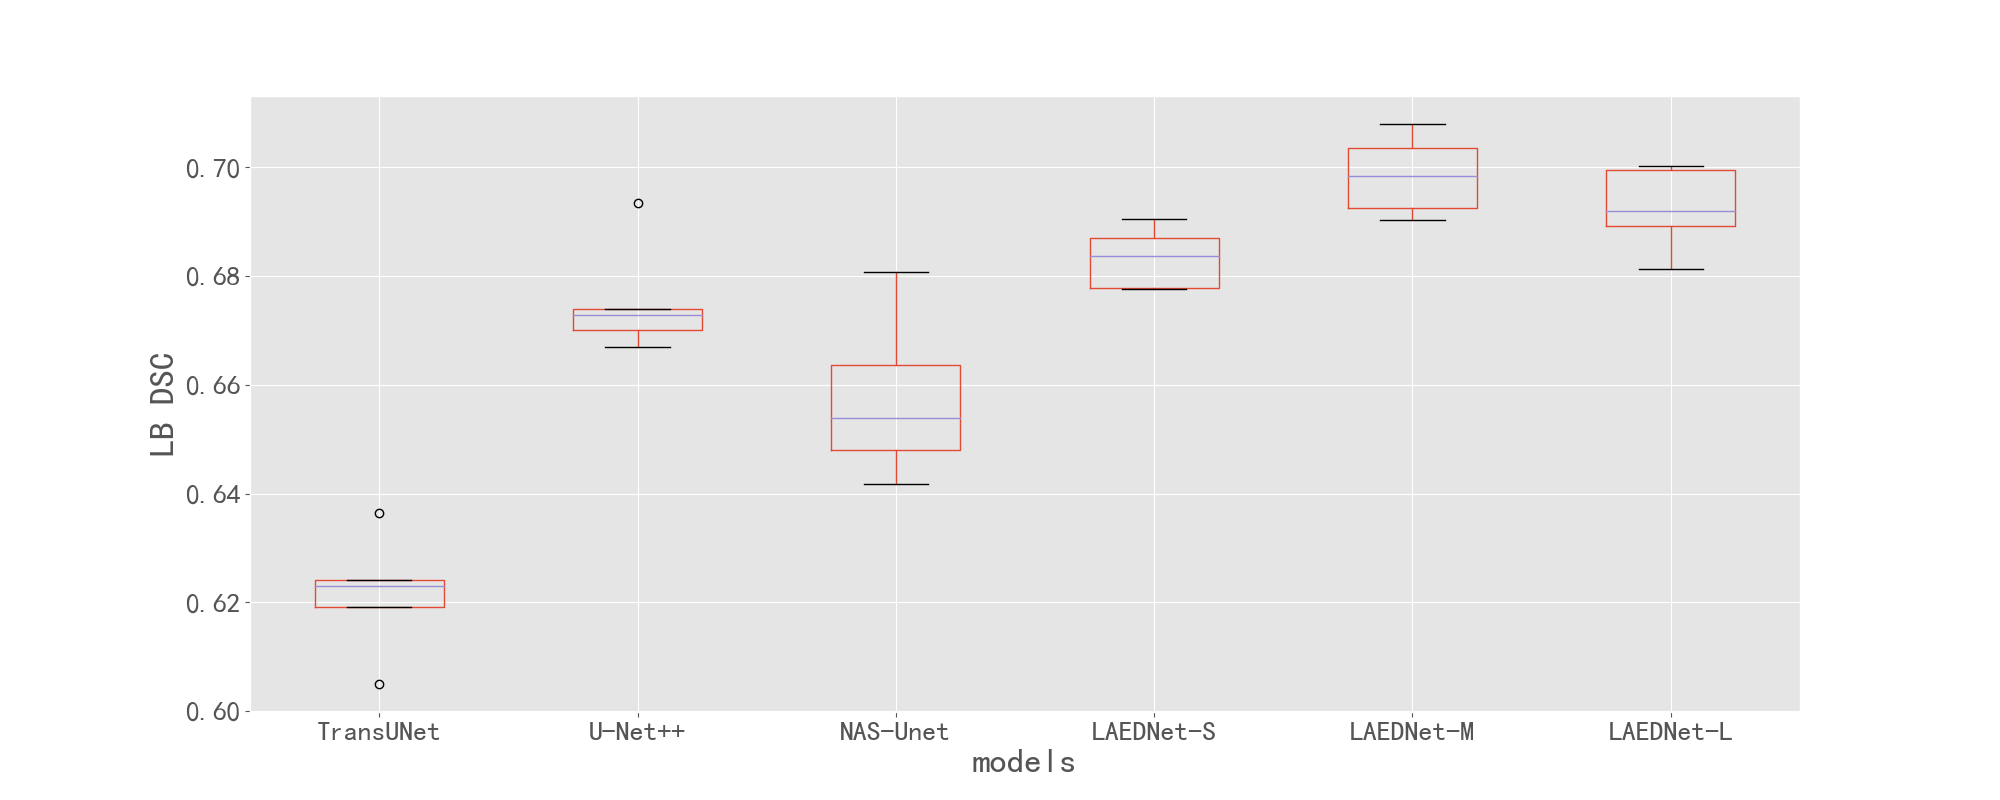
\includegraphics[width=1\linewidth]{boxplot-BP2.png}
	\centering
	\caption{Results of statistical experiments for U-Net++\cite{2020UNet}, TransUNet\cite{chen2021transunet}, NAS-Unet\cite{2019Nas-unet}, LAEDNet-S, LAEDNet-M and LAEDNet-L on BP\cite{Kaggle} dataset. (Best viewed in color)}
	\label{fig4}
\end{figure}

\emph{1) Results on BP}: Table \ref{table2} reports the Comparison results between state-of-the-art networks and LAEDNet on BP \cite{Kaggle} dataset. Our LAEDNet-M model achieves best trade-off between segmentation results and running speed. It only has 10.75M model parameters, yet obtains 69.8\% LB DSC, 73.0\% DSC, 68.9\% IoU, and 88.6\% AUC, respectively, with 40.7 FPS inference speed. LAEDNet-S is nearly 2.5 times smaller and 1.5 times faster with respect to LAEDNet-M. The segmentation accuracy, however, is only 68.1\%, 72.4\%, 68.4\%, and 88.3\% in terms of LB DSC, DSC, IoU, and AUC, respectively. Note LAEDNet-L is with 63.25M model size and only 17 FPS implementing speed, together with slightly performance drops in terms of LB DSC (0.6\%). Among the baselines, TransUNet\cite{chen2021transunet} is ranked at bottom in terms of segmentation accuracy, probably due to the shortage of training data. On the other hand, due to the powerful network architecture, U-Net++\cite{2020UNet} achieves best performance in terms of LB DSC, DSC, IoU , and AUC (67.5\%, 70.3\%, 66.4\%, and 83.9\%), respectively, but is with the sacrifice of larger model size(36.15M) and lowest running speed (21.5 FPS). Although NAS-Unet\cite{2019Nas-unet} has the smallest model size, yet it delivers poor segmentation accuracy than LAEDNet-S (2.6\%, 0.6\% and 13.6\% in terms of LB DSC, DSC and AUC, respectively).

Figure \ref{fig4} plots the boxplot results on BP\cite{Kaggle}, where U-Net++,\cite{2020UNet} TransUNet\cite{chen2021transunet} and NAS-Unet\cite{2019Nas-unet} are selected as baselines. As shown in Figure 4, our method, especially LAEDNet-M, achieves highest segmentation accuracy. Among all baselines, TransUNet\cite{chen2021transunet} ranks at bottom, only obtaining 62.1\% LB DSC. Additionally, NAS-Unet\cite{2019Nas-unet} has greatest standard deviation, indicating that it is vulnerable to fluctuations of training data.

Figure \ref{fig5} demonstrates the prediction results of U-Net\cite{2015U}, M-Net\cite{2018Joint}, U-Net++\cite{2020UNet}, TransUNet\cite{chen2021transunet}, LAEDNet-S, LAEDNet-M and LAEDNet-L on BP\cite{Kaggle}. It can be seen that our models can predict the shape of the target most similar to the ground truth, and the contour edge is smoother. In comparison, the contour edges of the target predicted by U-Net\cite{2015U}, M-Net\cite{2018Joint}, U-Net++\cite{2020UNet} and TransUNet\cite{chen2021transunet} are irregular. In addition, from the example in the penultimate row in Figure \ref{fig5}, some selected baselines (U-Net\cite{2015U} and M-Net\cite{2018Joint}) show relatively poor predictions for images that do not contain targets, while our method correctly classifies all pixels into backgrounds. In last row of Figure \ref{fig5}, we show one example of poor segmentation prediction. This is probably because the spatial texture of target is not easily distinguish from background that has many noise and spots.

\begin{figure}[!t]
	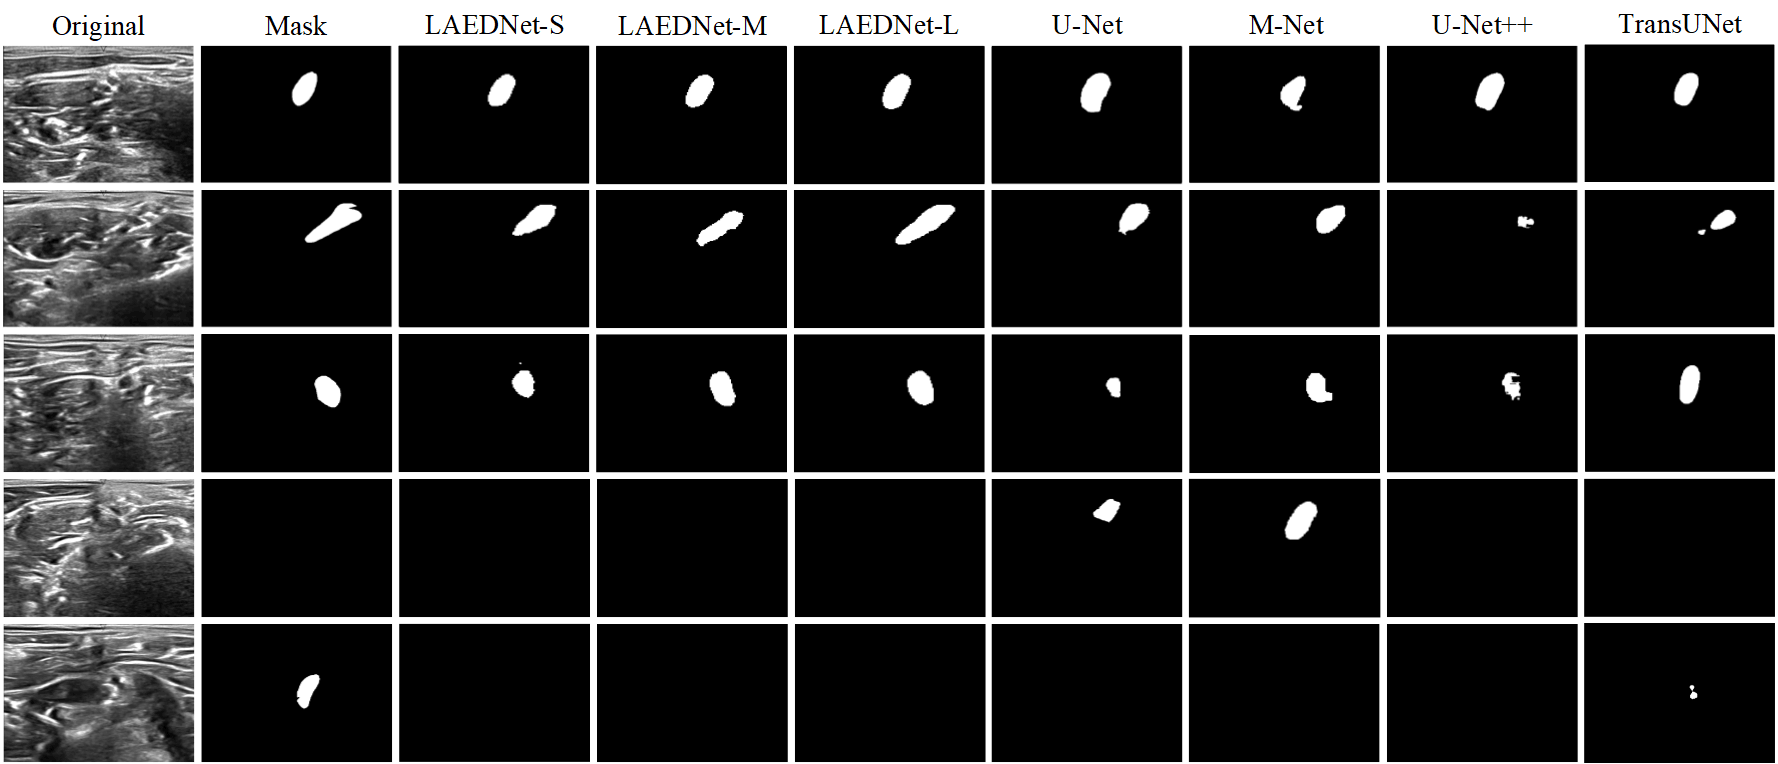
\includegraphics[width=\textwidth]{results-BP3.png}
	\centering
	\caption{Some visual examples of qualitative segmentation outputs on BP \cite{Kaggle} dataset. From left to right are results of U-Net\cite{2015U}, M-Net\cite{2018Joint}, U-Net++\cite{2020UNet}, TransUNet\cite{chen2021transunet}, LAEDNet-S, LAEDNet-M and LAEDNet-L. The last row shows an example of poor segmentation prediction. (Best viewed in color)}
	\label{fig5}
\end{figure}

\begin{table}[!t]
	\caption{Comparison results between state-of-the-art networks and LAEDNet on BUSI \cite{2019Dataset} dataset.}
	\centering
	\setlength{\tabcolsep}{3.2mm}
	\begin{tabular}{c|ccc|c|cc}
		\hline
		model & DSC(\%) & IoU(\%) & AUC(\%) & p-value &  Param(M) & FPS \\
		\hline
		U-Net \cite{2015U} & 63.2$\pm$1.1 & 54.2$\pm$3.9 & 84.5$\pm$2.0 & \textless0.001 & 28.97 & 30.7  \\
		\hline
		M-Net \cite{2019Deep} &	53.9$\pm$2.5 & 45.5$\pm$3.7 & 84.0$\pm$1.6 & \textless0.001 & 29.23 & 26.8 \\
		\hline
		U-Net++ \cite{2020UNet} & 70.9$\pm$1.8 & 63.8$\pm$2.7 & 90.4$\pm$1.3 & 0.201 & 36.15 & 21.5\\
		\hline
		TransUNet \cite{chen2021transunet} & 56.4$\pm$3.3 & 46.6$\pm$2.8 & 82.3$\pm$1.2 & \textless0.001 & 419.53 & 4.5 \\
		\hline
		SK-U-Net \cite{2020breastmass} & 72.4$\pm$2.4 & 65.5$\pm$4.4 & 86.4$\pm$2.5 & 0.394 & \textbf{3.94} & 19.6 \\
		\hline
		LAEDNet-S & 73.7$\pm$2.5 & 65.8$\pm$3.6 & 90.0$\pm$1.2 & 0.687 & 4.03 & \textbf{60.3} \\
		\hline
		LAEDNet-M & 73.8$\pm$1.3 & 65.8$\pm$2.0 & 91.0$\pm$0.5 & -- & 10.75 & 40.7 \\
		\hline
		LAEDNet-L & \textbf{75.0$\pm$0.9} & \textbf{67.6$\pm$3.4} & \textbf{91.3$\pm$1.1} & 0.353 & 63.25 & 17.0 \\
		\hline
	\end{tabular}\label{table3}
\end{table}

\begin{figure}[!t]
	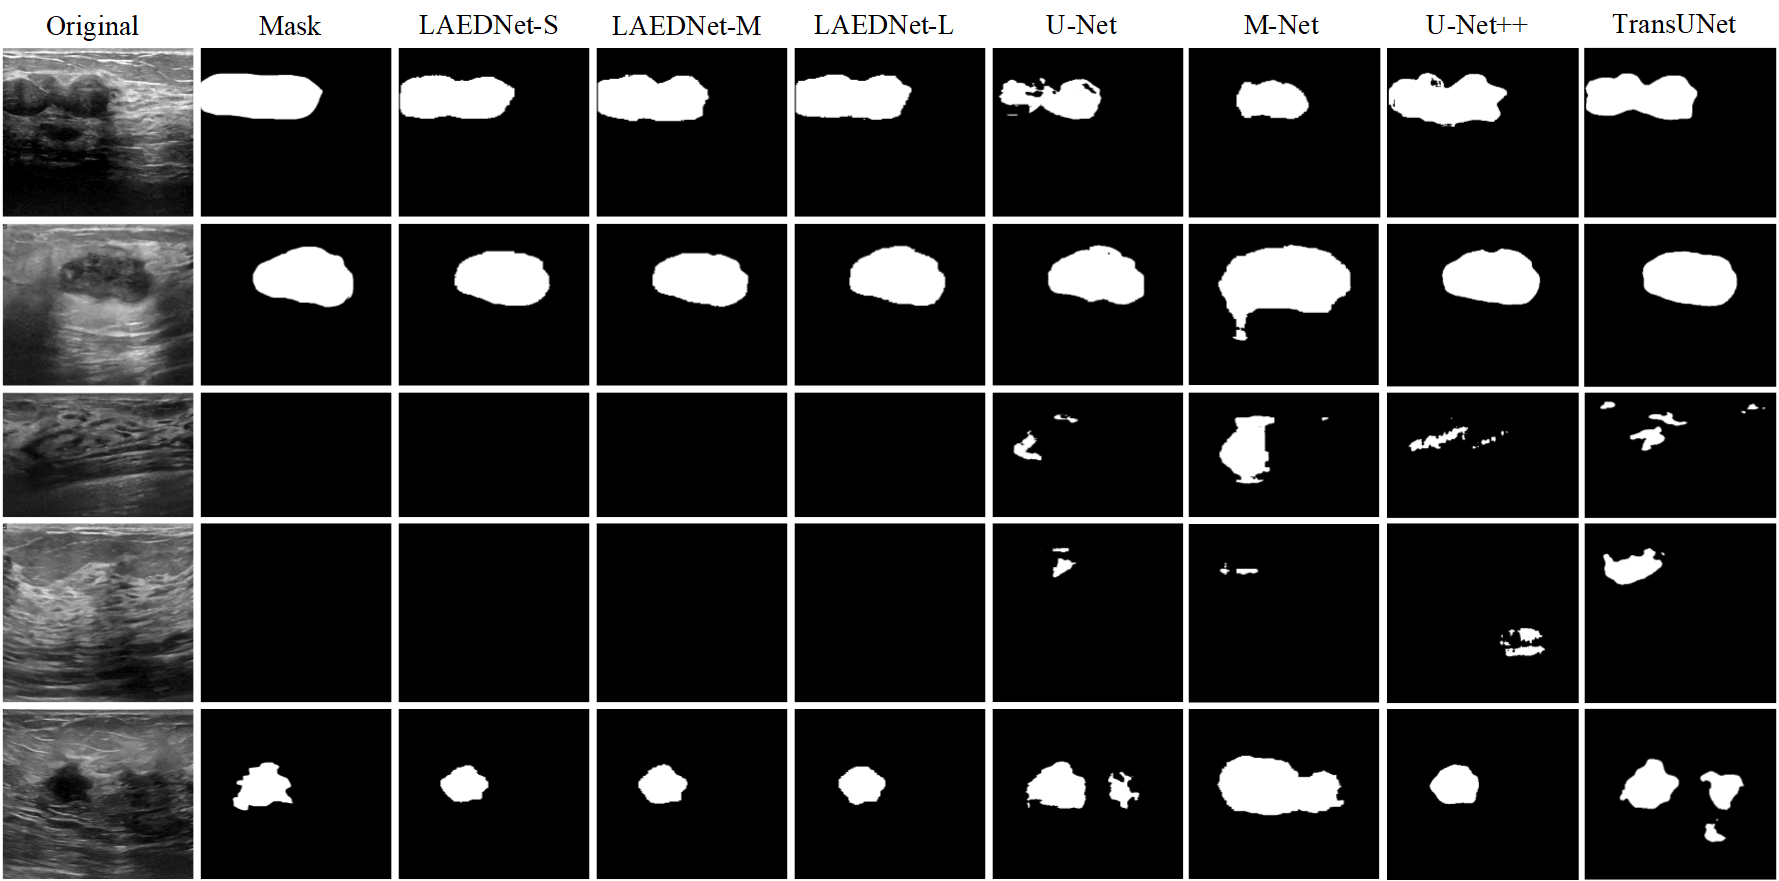
\includegraphics[width=\textwidth]{results-BUSI3.png}
	\caption{Some visual examples of qualitative segmentation outputs on BUSI \cite{2019Dataset} dataset. From left to right are results of U-Net\cite{2015U}, M-Net\cite{2018Joint}, U-Net++\cite{2020UNet}, TransUNet\cite{chen2021transunet}, LAEDNet-S, LAEDNet-M and LAEDNet-L. The last row shows an example of poor segmentation prediction. (Best viewed in color)}
	\label{fig6}
\end{figure}

\emph{2) Results on BUSI}: The quantitative results on BUSI\cite{2019Dataset} are reported in Table \ref{table3}. As can be seen, LAEDNet-S outperforms the U-Net++\cite{2020UNet} by 2.8\% and 2.0\% in DSC and IoU, respectively, while the AUC is slightly lower than U-Net++\cite{2020UNet}. LAEDNet-M outperforms the U-Net++\cite{2020UNet} by 2.9\%, 2.0\%, and 0.6\% in DSC, IoU, and AUC, respectively. And LAEDNet-L outperforms the U-Net++\cite{2020UNet} by 4.1\%, 3.8\%, and 0.9\% in DSC, IoU, and AUC, respectively. In spite of having smaller amount of parameters, SK-U-Net\cite{2020breastmass} performs slower (only 19.6 FPS) due to its fragmented operators. Besides, it obtains lower DSC, IOU and AUC scores than our LAEDNet. Specifically, LAEDNet improves the SK-U-Net\cite{2020breastmass} by a large margin of 1.3\%, 0.3\% and 3.6\%, respectively, in terms of DSC, IOU and AUC. Overall, LAEDNet-M achieves best trade-off between accuracy and efficiency. Note that since all input images are resized into $320\times320$, we obtain the same model parameters and FPS on BP\cite{Kaggle} and BUSI\cite{2019Dataset}. 

Figure \ref{fig6} shows the qualitative results of some visual examples on BUSI\cite{2019Dataset}. The results demonstrate that our LAEDNet is able to produce more fine segmentation results. The last row also exhibits a visual example of poor segmentation estimation. This is probably because that due to adhering to surrounding tissues, malignant tumors have irregular shapes and blurred boundaries, making them hard to be segmented. Even so, compared with selected baselines, the estimated outputs of LAEDNet are closer to the ground truth.

\begin{table}[!t]
	\caption{Comparison results between state-of-the-art networks and LAEDNet on HCUS \cite{2018Automated} dataset.}
	\centering
	\setlength{\tabcolsep}{3.3mm}
	\begin{tabular} {c|ccc|c|cc}
		\hline
		model & DSC(\%) & IoU(\%) & AUC(\%) & p-value &  Param(M) & FPS \\
		\hline
		U-Net \cite{2015U} & 82.8$\pm$0.9 & 73.8$\pm$2.0 & 96.8$\pm$0.8 & \textless0.001 & 28.97 & 30.7 \\
		\hline
		M-Net \cite{2019Deep} &	68.5$\pm$2.6 & 55.5$\pm$2.2 & 93.3$\pm$1.5 & \textless0.001 & 29.23 & 26.8 \\
		\hline
		U-Net++ \cite{2020UNet} & 88.9$\pm$1.8 & 82.6$\pm$2.1 & 98.4$\pm$0.8 & 0.106 & 36.15 & 21.5 \\
		\hline
		TransUNet \cite{chen2021transunet} & 75.8$\pm$3.2 & 64.8$\pm$2.6 & 91.0$\pm$2.4 & \textless0.001 & 419.53 & 4.5 \\
		\hline
		LAEDNet-S & 89.3$\pm$2.7 & 82.9$\pm$3.5 & 98.8$\pm$0.6 & 0.317 & \textbf{4.03} & \textbf{60.3} \\
		\hline
		LAEDNet-M & 91.3$\pm$2.2 & 85.6$\pm$2.4 & 99.0$\pm$0.3 & -- & 10.75 & 40.7 \\
		\hline
		LAEDNet-L & \textbf{91.7$\pm$1.5} & \textbf{86.1$\pm$2.5} & \textbf{99.1$\pm$0.4} & 0.722 & 63.25 & 17.0 \\
		\hline
	\end{tabular}\label{table4}
\end{table}

\begin{figure}[!t]
	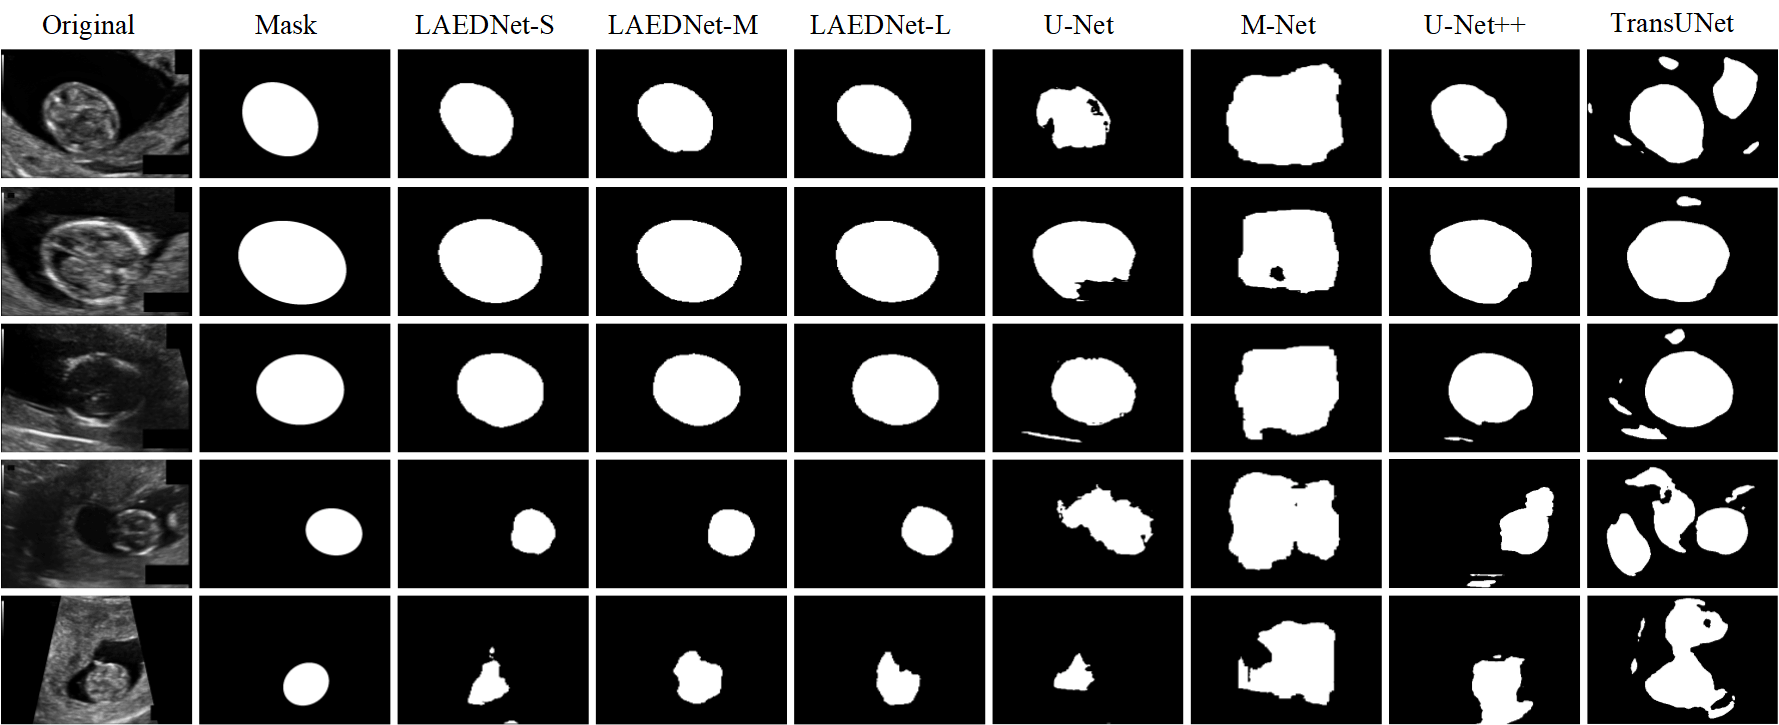
\includegraphics[width=\textwidth]{results-HCUS3.png}
	\caption{Some visual examples of qualitative segmentation outputs on HCUS \cite{2018Automated} dataset. From left to right are results of U-Net\cite{2015U}, M-Net\cite{2018Joint}, U-Net++\cite{2020UNet}, TransUNet\cite{chen2021transunet}, LAEDNet-S, LAEDNet-M and LAEDNet-L. The last row shows an example of poor segmentation prediction. (Best viewed in color)}
	\label{fig7}
\end{figure}

\emph{3) Results on HCUS}: Table \ref{table4} shows the results on HCUS\cite{2018Automated}, and compares with selected baselines. As can be seen, our method still achieves best performance on HCUS\cite{2018Automated}. In particular, compared with U-Net++\cite{2020UNet}, LAEDNet-S achieves 0.4\%, 0.3\%, and 0.4\% improvement in DSC, IoU, and AUC respectively. LAEDNet-M improves the results by 2.4\%, 3.0\%, and 0.6\% in DSC, IoU, and AUC, respectively. LAEDNet-L can achieve 91.7\% DSC, 86.1\% IoU, and 99.1\% AUC, which outperforms previous networks by a large margin. The model parameters and the FPS are the same as those on BP\cite{Kaggle} and BUSI\cite{2019Dataset}. The results demonstrate that our networks not only achieve significant improvements in segmentation accuracy, but also lead to great reduction of network parameters. Several visual examples of segmentation outputs are shown in Figure 7. Compared with previous models, our networks show outstanding segmentation capabilities on HCUS\cite{2018Automated}.

\section{Discussion}

Although the focus of this paper is to segment target region in ultrasound image, the segmentation results are truly useful for clinical diagnose. As shown in the experimental results, LAEDNet can segment the neurons or lesions in the ultrasound image in a timely fashion. This is very helpful to ensure the success of operations such as anesthesia injection or ultrasound puncture by the doctor. In particular, in the detection of masses, such as the detection of breast nodules, LAEDNet can segment objects with clear boundaries from low-contrast images, so that doctors can judge whether it is benign or malignant according to the shape of the segmented mass.

To further verify the contributions of LRSE--SE module in decoder PUS training strategy, we carry on ablation studies on BP\cite{Kaggle} dataset using LAEDNet-M, as it can achieves best trade-off between segmentation accuracy and implementing efficiency. As we have mentioned in Section \ref{dataset}, the region area of neuron target is relatively small with respect to the entire image, and BP datset even contains a large number of images without neuron targets, thus leading to unbalanced distribution of training samples in the dataset. To resolve this problem, we resort to PUS. For fair comparison with SE module, it is also repeatedly performed 5 times along with SE introduced. The experimental results are shown in Table \ref{ablation}.

\begin{table}[!t]
	\caption{The results of ablation experiments.}
	\centering
	\setlength{\tabcolsep}{1.5mm}
	\begin{tabular} {c|cc|cccc|c|c}
		\hline
		model & SE & PUS & LB DSC(\%) & DSC(\%) & IoU(\%) & AUC(\%) & p-value & Param(M) \\
		\hline
		LAEDNet-M & & & 67.4$\pm$1.2 & 71.8$\pm$0.9 & 68.0$\pm$1.0 & 84.8$\pm$0.6 & 0.005 & 10.45\\
		\hline
		LAEDNet-M & \checkmark & & 68.2$\pm$0.6 & 72.2$\pm$0.8 & 68.2$\pm$0.7 & 86.1$\pm$1.0 & 0.006 & 10.75\\
		\hline
		LAEDNet-M &	\checkmark & \checkmark & \textbf{69.8$\pm$0.6} & \textbf{73.0$\pm$0.4} & \textbf{68.9$\pm$0.4} & \textbf{88.6$\pm$0.4} & -- & 10.75\\
		\hline
	\end{tabular}
	\label{ablation}
\end{table}

As we can seen from Table \ref{ablation}, SE only brings 0.3M increase of model size, yet it averagely yields 0.8\%, 0.4\%, 0.2\% and 1.3\% improvement of LB DSC, DSC, IoU and AUC score, respectively, demonstrating the effectiveness of SE. On the other hand, Table \ref{ablation} shows that the performance boosts 1.6\%, 0.8\%, 0.7\% and 2.5\%, respectively, using PUS training strategy, indicating that PUS well addresses unbalance issue of training data. The qualitative results are shown in Figure \ref{fig8}, where Model-1 represents the baseline without SE module and PUS, and model-2 represents the model with SE but without PUS. As shown in Figure \ref{fig8}, compared with baseline, employing SE produces better segmentation outputs. When PUS training strategy is introduced, our LAEDNet-M is able to yield more consistent segmentation results with ground truth.

\begin{figure}[!t]
	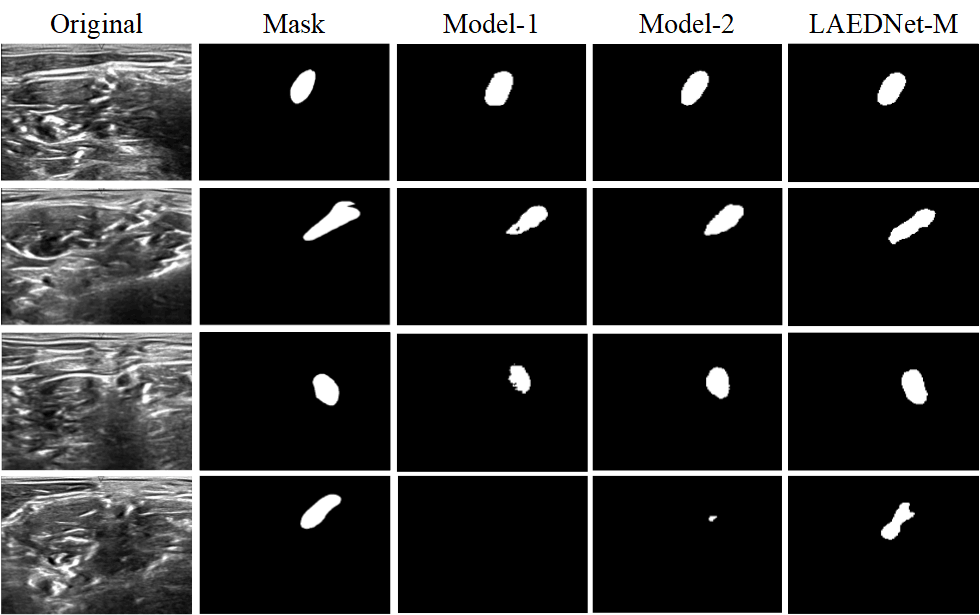
\includegraphics[width=\textwidth]{results-ablation1.png}
	\caption{Sample test predictions of Model-1(without SE module or PUS), Model-2(With SE module but without PUS) and LAEDNet-M on BP\cite{Kaggle}. The last row is the worst segmentation results on BP\cite{Kaggle}. (Best viewed in color)}
	\label{fig8}
\end{figure}

Finally, to show whether the differences between algorithms are statistically significant, we have also conducted t-test on the results and reported p-values from Table \ref{table2} to Table \ref{table4}. More specifically, for all datasets, the p-value is computed from each segmentation network with respect to LAEDNet-M model. It is worth to mention that, for BP dataset, we report p-value from the metric of LB DSC, as it is used to evaluate segmentation results on test set. While for other two datsets, we report averaged p-value from the metrics of DSC, IoU and AUC, respectively, as these metrics are used on validation set.

From Table \ref{table2}, it is evident that, except LAEDNet-L, our LAEDNet-M model is significantly different from selected baselines. We also observe similar results in ablation study, as shown in Table \ref{ablation}. However, as shown in Table \ref{table3} and Table \ref{table4}, it is interesting that the most similar models with respect to LAEDNet-M are LAEDNet-S and LAEDNet-L on BUSI and HCUS datasets, respectively. Furthermore, the p-value of HCUS dataset is 0.722, indicating that our LAEDNet-M model achieves similar performance with high accuracy model, yet with fewer model size and higher running speed.

\section{Conclusion}

In this paper, we have presented a novel asymmetrical encoder-decoder architecture, LAEDNet, to achieve best available trade-off between segmentation accuracy and implementing efficiency for ultrasound image segmentation. We have adopted 3 versions of EfficientNet as encoder to construct 3 versions of LAEDNet. A set of LRSEs are designed to couple with encode, where channel-wised attention is adopted to integrate decoding features and counterpart features in encoder. To evaluate our models, the experiments are conducted on three challenging datasets: BP\cite{Kaggle}, BUSI\cite{2019Dataset} and HCUS\cite{2018Automated}. The experimental results demonstrate that our LAEDNet outperforms U-Net\cite{2015U}, M-Net\cite{2018Joint}, U-Net++\cite{2020UNet}, TransUNet\cite{chen2021transunet}, and other lightweight networks\cite{2019Nas-unet,2020breastmass}, in terms of segmentation accuracy. Besides, our LAEDNet-M achieves best trade-off in terms of segmentation accuracy and implementing efficiency on three datasets. We have also proved the validity of PUS training strategy and the SE module in LRSE through ablation studies. In the future, we will explore the possibility of more lightweight encoder instead of using EfficientNet. We are also interesting in applying our model to video sequence, which facilitate to online medical diagnose.

\section*{Acknowledgment}

This work was jointly supported in part by the National Natural Science Foundation of China under Grants 61876093, 61871234, China Postdoctoral Science Foundation Funded Project under Grant 2020M671595, and Post-doctoral Science Foundation of Jiangsu Province under Grant 2020Z198.

\section*{References}

\bibliography{mybibfile}

\section*{Short bio}

\textbf{Quan Zhou} received Ph.D. degree in electronics and information engineering from Huazhong University of Science and Technology, Wuhan, China in 2013. Now he is an associated professor in the college of Telecommunications and Information engineering at Nanjing University of Posts and Telecommunications. His research interests include computer vision and pattern recognition.

\textbf{Qianwen Wang} received B.S. degree in information engineering from Nanjing University of Posts and Telecommunications. She is now pursuing her master degree in Nanjing University of Posts and Telecommunications. Her research interests include medical image segmentation.

\textbf{Yuncao Bao} received B.S. degree in information engineering from Nanjing University of Posts and Telecommunications. He is now pursuing his master degree in Nanjing University of Posts and Telecommunications. Her research interests include medical image segmentation.

\textbf{Linjun Kong} is now served as a full professor in Jingling Institute of Technology. His research interests include  computer vision and pattern recognition.

\textbf{Xin Jin} received Ph.D. degree from Beihang University. Now he is an associated professor in the department of computer science and technology, Beijing Electronic Science and Technology Institute. His research interests include computer vision and pattern recognition.

\textbf{Weihua Ou} received Ph.D. degree from Huazhong University of Science and Technology, Wuhan, China. Now he is a full professor in the School of Big data and computer science, Guizhou Normal University. His research interests include computer vision and pattern recognition.

\end{document}